% GENERATED by tools/render_sysml_diagrams.py. Do not edit: the next run overwrites it.
% To change a caption, edit the `// caption:` line above the view in the .sysml file.
% To explain a diagram, add `// note:` lines there; they follow the caption.
% To add or remove a figure, add or remove the view in the model.
% To move a figure between the body and the appendix, add or remove a
% `// placement: body` line above the caption line.

\begin{landscape}
\begin{figure}[!htbp]
\centering
\pdfimageresolution=300
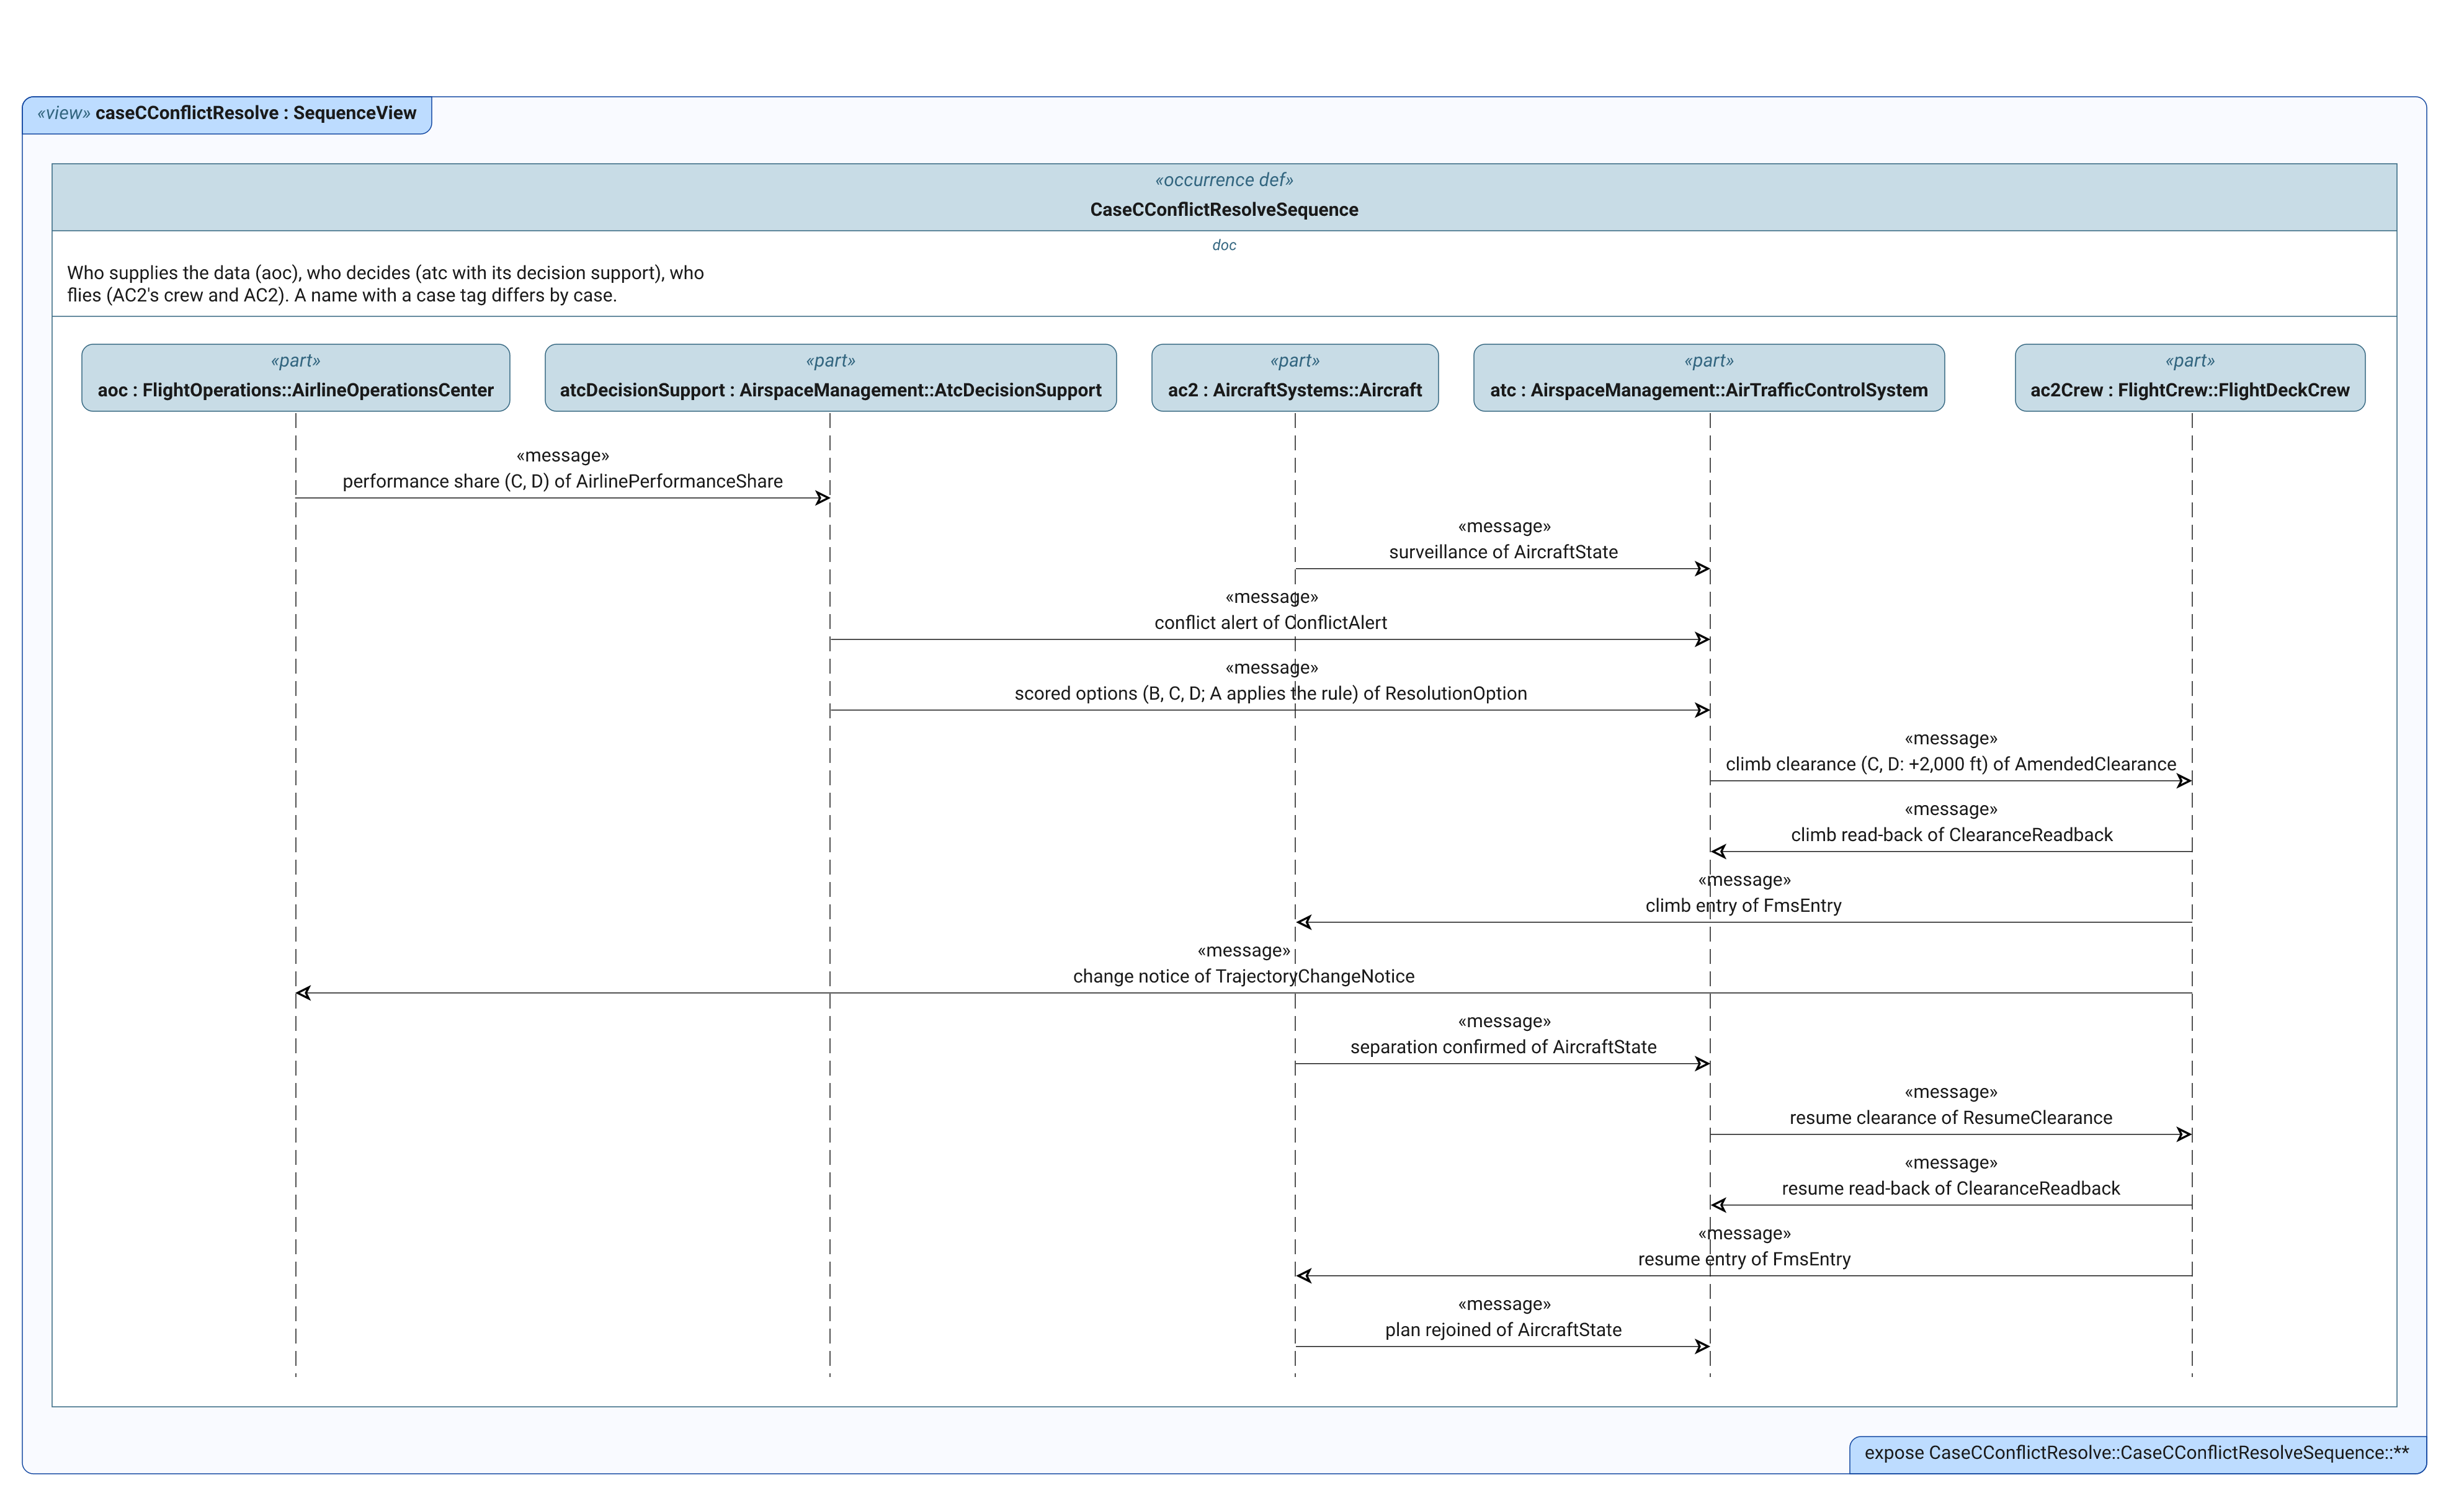
\includegraphics[width=\linewidth,height=0.8\textheight,keepaspectratio]{sysml/diagram-caseCConflictResolve}
\caption[Case C Conflict Resolve: the exchanges when ATC decision support scores the options with the airline's shared data]{Case C Conflict Resolve: the exchanges when ATC decision support scores the options with the airline's shared data. The atcDecisionSupport lifeline is ATC's decision support, the En Route Decision Support Tool (EDST; FAA JO 7110.65BB, para. 13-1-1). EDST raises the conflict alert today; scoring the resolution options with the airline's shared data is the proposed improvement. View \texttt{caseCConflictResolve}; source \texttt{nas\_sequence\_case\_c.sysml}; rendered 2026-11-05.}
\label{fig:sysml-caseCConflictResolve}
\end{figure}
\end{landscape}
